
\chapter{Methodology}

In this section, the methodology to perform our experiments is described. The goal of our experiments is to gain compact and expressive audio embeddings in an efficient manner. Toward this goal, our methodology handles audio and text data effectively so that a neural model learns sound representations using two modals of information. 

Our experiment process is divided into four steps: Data collection, Pre-processing, model training and feature extraction, and evaluation. 

% All the input audio data are collected from Freesound.org. Each audio file should have a single or multiple tags which describe the sound content in textual format. In pre-processing, each audio file are converted to a spectrogram in a fixed width and height which is then fed to a neural network model. During the training of the model, the parameters of the neural network are updated using a batch. The trained model, then, is evaluated by both objective and subjective measures.

\begin{figure}[htb]
	\centering
	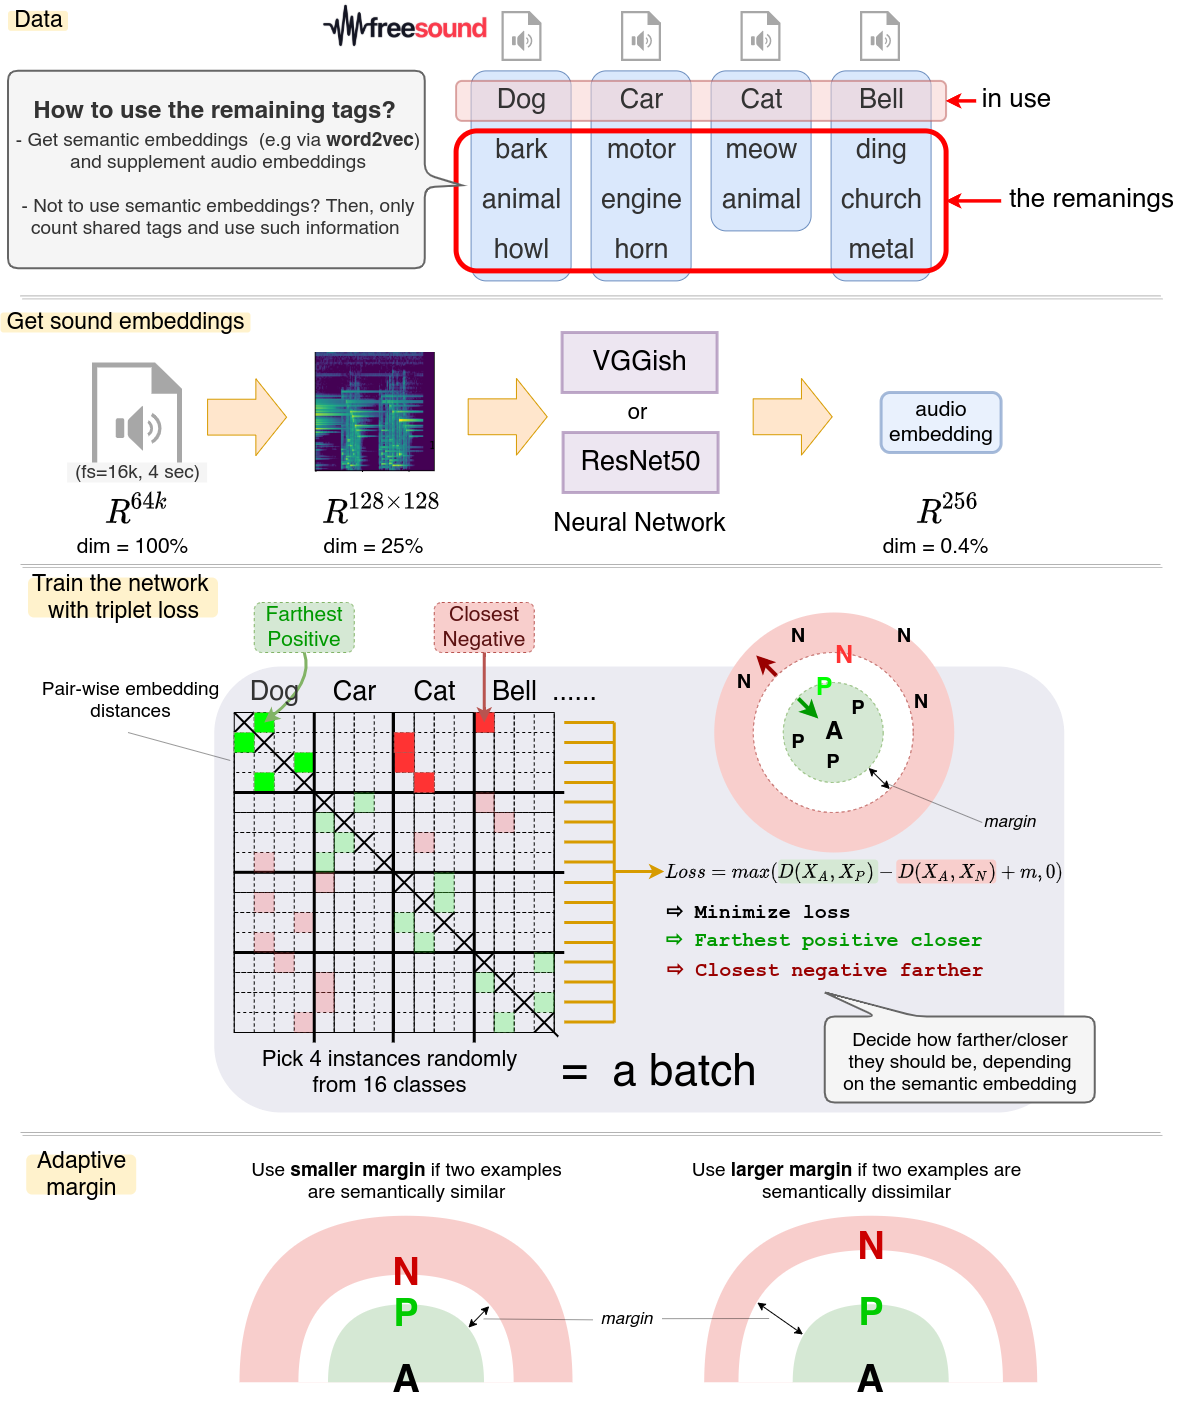
\includegraphics[width=15cm]{Figures/Triplet-Loss_Semantic.png}
	\caption{Experiment overview. The diagram is correct but needs to be updated to correspond to the explanation in the thesis.}
	\label{toc-figrue}
\end{figure}

\clearpage

\section{Data collection}
The dataset we used are built solely based on audio data and its associated tags freely available on Freesound.org. To download efficiently from the website, we developed a script\footnote{\texttt{https://github.com/kokimame/OpenFSE/blob/master/src/utils/freesound\_200k\_dl.py}} which download sounds as a batch using Freesound APIv2 and its Python client service. In total, we downloaded about 200K sounds and stored them in the MP3 format. The sounds we downloaded are determined so that the total number of the tags associated with the sounds becomes 500. All the sound are sampled at 16,000 Hz and have duration between XXX seconds at minimum and XXX seconds at maximum.

As the nature of Freesound.org, most of sound data are associated with more than one labels. We want to preserve the multi-labelled nature since it provides more text description of sounds than single-labeled dataset and helps our model learn semantically-rich representations. 

Unlike the cases of single-labeled dataset where a label of sound data is explained simply in its file name or parent directory, we store the multi-label relationship in a CSV\footnote{\texttt{https://github.com/kokimame/OpenFSE/blob/master/src/data/tags\_ppc\_top\_500.csv}}. This information will be read in the training of our model and be used to tell whether each pair of sounds have any label in common.

% Explanation on Multilabel statistics and Balanced Data
% No. balancing should be discussed earlier
Our dataset consists of 15,000 sound data that covers 500 classes (labels) of sounds and that are licensed under Creative Commons. Each class of sounds has 30 sound instances. While balancing multi-labeled data possibly screws the nature of its data, we had to do balancing our dataset to this extent because our GPU does not have enough memory to handle all the data we could have and we could not develop a workaround for the lack of GPU memory. 

In our multi-labeled dataset, there are XXX sound data and 500 labels are observed in total. Each sound data has XXX labels on average while the top 3 labels that are observed the most were XXX (XXX), XXX (XXX), and XXX (XXX). As you can see in Figure 4, the variety of the types of labels is diverse. For example, labels related to music instrument such as XXX appears XXX while labels like XXX which is related to nature sound appears as frequently as the former one.

\section{Pre-Processing}
Each sound in the MP3 format is converted to a sequence of spectrograms. To analyze the frequency components of audio, each audio recordings are divided into a set of short audio waveforms of 4 seconds. Based on each of the waveforms, we compute 128-channel mel-scale spectrograms using an FFT window size of 64 ms with 32 ms step. We limit the power of spectrograms between -80 db to 0 db and then normalize it between 0 and 1. In the end, the waveform of 4 seconds are turned into a 128x128 spectrogram which is an input to our following neural network.

The spectrograms are stored in a \texttt{.pt} file for serialization along with corresponding label and original sound ID on Freesound. For the dataset file for training, the size of this serialized file becomes about 130MB, and this file will be loaded in the beginning of the model training process.

\section{Model Training}
\subsection{Network Architecture}

In our work, neural network is used in the process that transforms 2 dimensional audio representations (spectrogram) to smaller 1 dimensional vectors. Similar to the nonlinear approach traditionally used in this part such as MFCCs, our neural network has to be powerful enough to learn the nonlinear transformation yet efficient enough to perform this process quickly.

Our strategy to find a right network architecture for our task is that first we find successful architecture in the task similar to ours from previous work and re-implement their model with minimal modifications, and then, after conducting experiments to analyze the model performance in our task, we modify and improve the architecture of the network.

Following this strategy, we first employ the VGG-based architecture used in~\cite{hershey2017} because of its capacity to perform well in large-scale audio classification and its simplicity of implementation.

% Visualize the architecture

\section{Training Strategy}
Our model is trained while updating the network's weights by backward propagation of its prediction error. The prediction error in the output layer of the network is computed based on the triplet loss formula (See Section 2.X for the detail of the triplet loss function) given by
\begin{equation}
    L = \max(D(X_A, X_P) - D (X_A, X_N ) + m, 0) 
\end{equation}
using the distance function
\begin{equation}
    D(X_i, X_j) = \frac{1}{d} || f(X_i) - f(X_j)||
\end{equation}

where $m$ is a value that defines the margin between positive instances and negative instances.

We train our network for 10 epochs and run a validation process to obtain mAP scores using the latest saved models. We use plain stochastic gradient descent to optimize our model with a constant learning rate of 0.1. While we could make use of more complex training strategy such as the use of scheduled learning rate or more advanced optimizers, we decided not to go into the detail of this configuration and development because our main concern is to investigate similarity learning instead of achieving a state-of-the-art performance.

\subsection{Triplet Mining}
As discussed in the last chapter, the way of choosing the triplets in each mini-batch has significant effects on learning performance. For our study, we chose an online semi-hard mining strategy. In our implementation, we choose 5 unique labels and 4 sound instances per label, forming a mini-batch of 20.

\newpage

\section{Adaptive Margin}
Most deep metric learning algorithms, which only use coarse-grained sound classes, fail to learn distances that capture fine-grained sub-categories. Such fine-grained audio similarity distances are important to learn generalized visual features and to have robust performance on cross-domain data (e.g., both urban sound data and music instrument data).

To increase the granularity of the target sound classes, we employ the multiple tags associated to each sound data on Freesound. This expands the size of the classes and the difference of the similarity becomes more evident among the pairs of the classes. For example, the pair of the tags such as 'Speech' and 'Bark' is more similar with each other than the pair of 'Horn' and 'Bark' since 'Speech' and 'Bark' are probably produced from living creatures.

To utilize more semantic content of the tags, we employ semantic vectors to adjust the margin of the triplet loss.

\begin{itemize}
    \item If two sounds belong to semantically similar labels, no need to push two representation too much. Therefore, we use a smaller margin. Otherwise, we use a large margin.
    \item For example, given an anchor with label "Bark", if we compare negative instances with label "Speech" and with label "Car", we want to push the instance of "Car" farther than "Speech" from the anchor. This is because "Bark" and "Speech" are more semantically similar (both sounds are produced from living creatures even though perceptually quite different) than the other combination.
\end{itemize}

\begin{figure}[htb]
	\centering
	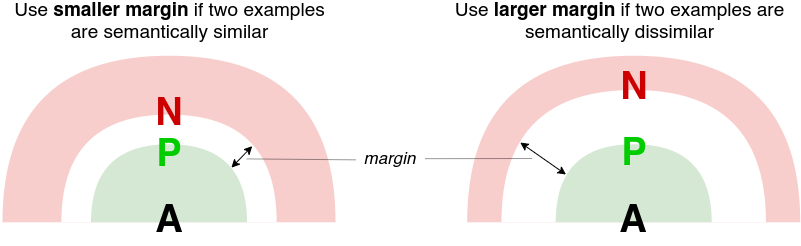
\includegraphics[width=15cm]{Figures/Adaptive_Margin.png}
	\caption{Experiment overview. The diagram is correct but needs to be updated to correspond to the explanation in the thesis.}
	\label{toc-figrue}
\end{figure}
